% Figure from MATH 556 notes, section 2. Compile with the notes preamble.
\definecolor{axlerblue}{RGB}{200, 220, 240}
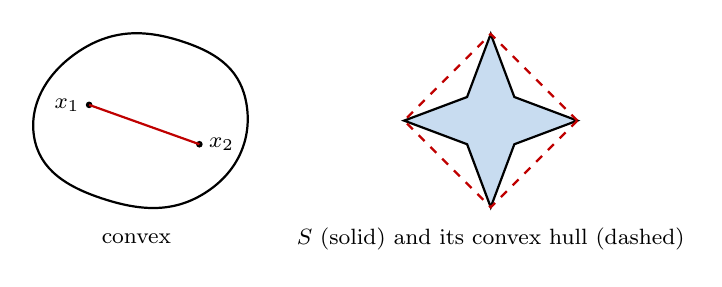
\begin{tikzpicture}[scale=1.0, >=stealth]
    % convex blob
    \begin{scope}
        \draw[thick] plot[smooth cycle, tension=0.8] coordinates {(-1.3,-0.2) (-0.7,0.9) (0.6,1.0) (1.4,0.2) (0.9,-0.9) (-0.4,-1.0)};
        \fill (-0.6,0.2) circle (1.2pt) node[left, font=\footnotesize] {$x_1$};
        \fill (0.8,-0.3) circle (1.2pt) node[right, font=\footnotesize] {$x_2$};
        \draw[thick, red!75!black] (-0.6,0.2) -- (0.8,-0.3);
        \node[font=\footnotesize] at (0,-1.5) {convex};
    \end{scope}
    % star and its hull
    \begin{scope}[xshift=4.5cm]
        \fill[axlerblue] (1.1,0) -- (0.3,0.3) -- (0,1.1) -- (-0.3,0.3) -- (-1.1,0) -- (-0.3,-0.3) -- (0,-1.1) -- (0.3,-0.3) -- cycle;
        \draw[thick] (1.1,0) -- (0.3,0.3) -- (0,1.1) -- (-0.3,0.3) -- (-1.1,0) -- (-0.3,-0.3) -- (0,-1.1) -- (0.3,-0.3) -- cycle;
        \draw[dashed, thick, red!75!black] (1.1,0) -- (0,1.1) -- (-1.1,0) -- (0,-1.1) -- cycle;
        \node[font=\footnotesize] at (0,-1.5) {$S$ (solid) and its convex hull (dashed)};
    \end{scope}
\end{tikzpicture}
